\documentclass[1p]{elsarticle_modified}
%\bibliographystyle{elsarticle-num}

%\usepackage[colorlinks]{hyperref}
%\usepackage{abbrmath_seonhwa} %\Abb, \Ascr, \Acal ,\Abf, \Afrak
\usepackage{amsfonts}
\usepackage{amssymb}
\usepackage{amsmath}
\usepackage{amsthm}
\usepackage{scalefnt}
\usepackage{amsbsy}
\usepackage{kotex}
\usepackage{caption}
\usepackage{subfig}
\usepackage{color}
\usepackage{graphicx}
\usepackage{xcolor} %% white, black, red, green, blue, cyan, magenta, yellow
\usepackage{float}
\usepackage{setspace}
\usepackage{hyperref}

\usepackage{tikz}
\usetikzlibrary{arrows}

\usepackage{multirow}
\usepackage{array} % fixed length table
\usepackage{hhline}

%%%%%%%%%%%%%%%%%%%%%
\makeatletter
\renewcommand*\env@matrix[1][\arraystretch]{%
	\edef\arraystretch{#1}%
	\hskip -\arraycolsep
	\let\@ifnextchar\new@ifnextchar
	\array{*\c@MaxMatrixCols c}}
\makeatother %https://tex.stackexchange.com/questions/14071/how-can-i-increase-the-line-spacing-in-a-matrix
%%%%%%%%%%%%%%%

\usepackage[normalem]{ulem}

\newcommand{\msout}[1]{\ifmmode\text{\sout{\ensuremath{#1}}}\else\sout{#1}\fi}
%SOURCE: \msout is \stkout macro in https://tex.stackexchange.com/questions/20609/strikeout-in-math-mode

\newcommand{\cancel}[1]{
	\ifmmode
	{\color{red}\msout{#1}}
	\else
	{\color{red}\sout{#1}}
	\fi
}

\newcommand{\add}[1]{
	{\color{blue}\uwave{#1}}
}

\newcommand{\replace}[2]{
	\ifmmode
	{\color{red}\msout{#1}}{\color{blue}\uwave{#2}}
	\else
	{\color{red}\sout{#1}}{\color{blue}\uwave{#2}}
	\fi
}

\newcommand{\Sol}{\mathcal{S}} %segment
\newcommand{\D}{D} %diagram
\newcommand{\A}{\mathcal{A}} %arc


%%%%%%%%%%%%%%%%%%%%%%%%%%%%%5 test

\def\sl{\operatorname{\textup{SL}}(2,\Cbb)}
\def\psl{\operatorname{\textup{PSL}}(2,\Cbb)}
\def\quan{\mkern 1mu \triangleright \mkern 1mu}

\theoremstyle{definition}
\newtheorem{thm}{Theorem}[section]
\newtheorem{prop}[thm]{Proposition}
\newtheorem{lem}[thm]{Lemma}
\newtheorem{ques}[thm]{Question}
\newtheorem{cor}[thm]{Corollary}
\newtheorem{defn}[thm]{Definition}
\newtheorem{exam}[thm]{Example}
\newtheorem{rmk}[thm]{Remark}
\newtheorem{alg}[thm]{Algorithm}

\newcommand{\I}{\sqrt{-1}}
\begin{document}

%\begin{frontmatter}
%
%\title{Boundary parabolic representations of knots up to 8 crossings}
%
%%% Group authors per affiliation:
%\author{Yunhi Cho} 
%\address{Department of Mathematics, University of Seoul, Seoul, Korea}
%\ead{yhcho@uos.ac.kr}
%
%
%\author{Seonhwa Kim} %\fnref{s_kim}}
%\address{Center for Geometry and Physics, Institute for Basic Science, Pohang, 37673, Korea}
%\ead{ryeona17@ibs.re.kr}
%
%\author{Hyuk Kim}
%\address{Department of Mathematical Sciences, Seoul National University, Seoul 08826, Korea}
%\ead{hyukkim@snu.ac.kr}
%
%\author{Seokbeom Yoon}
%\address{Department of Mathematical Sciences, Seoul National University, Seoul, 08826,  Korea}
%\ead{sbyoon15@snu.ac.kr}
%
%\begin{abstract}
%We find all boundary parabolic representation of knots up to 8 crossings.
%
%\end{abstract}
%\begin{keyword}
%    \MSC[2010] 57M25 
%\end{keyword}
%
%\end{frontmatter}

%\linenumbers
%\tableofcontents
%
\newcommand\colored[1]{\textcolor{white}{\rule[-0.35ex]{0.8em}{1.4ex}}\kern-0.8em\color{red} #1}%
%\newcommand\colored[1]{\textcolor{white}{ #1}\kern-2.17ex	\textcolor{white}{ #1}\kern-1.81ex	\textcolor{white}{ #1}\kern-2.15ex\color{red}#1	}

{\Large $\underline{12a_{0237}~(K12a_{0237})}$}

\setlength{\tabcolsep}{10pt}
\renewcommand{\arraystretch}{1.6}
\vspace{1cm}\begin{tabular}{m{100pt}>{\centering\arraybackslash}m{274pt}}
\multirow{5}{120pt}{
	\centering
	\includegraphics[width=112pt]{../../../GIT/diagram.site/Diagrams/png/1038_12a_0237.png}\\
\ \ \ A knot diagram\footnotemark}&
\allowdisplaybreaks
\textbf{Linearized knot diagam} \\
\cline{2-2}
 &
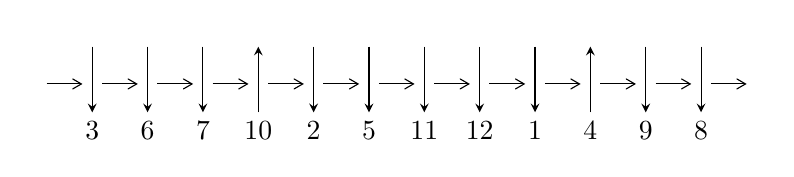
\begin{tikzpicture}[x=20pt, y=17pt]
	% nodes
	\node (C0) at (0, 0) {};
	\node (C1) at (1, 0) {};
	\node (C1U) at (1, +1) {};
	\node (C1D) at (1, -1) {3};

	\node (C2) at (2, 0) {};
	\node (C2U) at (2, +1) {};
	\node (C2D) at (2, -1) {6};

	\node (C3) at (3, 0) {};
	\node (C3U) at (3, +1) {};
	\node (C3D) at (3, -1) {7};

	\node (C4) at (4, 0) {};
	\node (C4U) at (4, +1) {};
	\node (C4D) at (4, -1) {10};

	\node (C5) at (5, 0) {};
	\node (C5U) at (5, +1) {};
	\node (C5D) at (5, -1) {2};

	\node (C6) at (6, 0) {};
	\node (C6U) at (6, +1) {};
	\node (C6D) at (6, -1) {5};

	\node (C7) at (7, 0) {};
	\node (C7U) at (7, +1) {};
	\node (C7D) at (7, -1) {11};

	\node (C8) at (8, 0) {};
	\node (C8U) at (8, +1) {};
	\node (C8D) at (8, -1) {12};

	\node (C9) at (9, 0) {};
	\node (C9U) at (9, +1) {};
	\node (C9D) at (9, -1) {1};

	\node (C10) at (10, 0) {};
	\node (C10U) at (10, +1) {};
	\node (C10D) at (10, -1) {4};

	\node (C11) at (11, 0) {};
	\node (C11U) at (11, +1) {};
	\node (C11D) at (11, -1) {9};

	\node (C12) at (12, 0) {};
	\node (C12U) at (12, +1) {};
	\node (C12D) at (12, -1) {8};
	\node (C13) at (13, 0) {};

	% arrows
	\draw[->,>={angle 60}]
	(C0) edge (C1) (C1) edge (C2) (C2) edge (C3) (C3) edge (C4) (C4) edge (C5) (C5) edge (C6) (C6) edge (C7) (C7) edge (C8) (C8) edge (C9) (C9) edge (C10) (C10) edge (C11) (C11) edge (C12) (C12) edge (C13) ;	\draw[->,>=stealth]
	(C1U) edge (C1D) (C2U) edge (C2D) (C3U) edge (C3D) (C4D) edge (C4U) (C5U) edge (C5D) (C6U) edge (C6D) (C7U) edge (C7D) (C8U) edge (C8D) (C9U) edge (C9D) (C10D) edge (C10U) (C11U) edge (C11D) (C12U) edge (C12D) ;
	\end{tikzpicture} \\
\hhline{~~} \\& 
\textbf{Solving Sequence} \\ \cline{2-2} 
 &
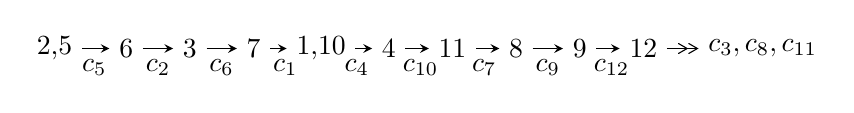
\begin{tikzpicture}[x=23pt, y=7pt]
	% node
	\node (A0) at (-1/8, 0) {2,5};
	\node (A1) at (1, 0) {6};
	\node (A2) at (2, 0) {3};
	\node (A3) at (3, 0) {7};
	\node (A4) at (65/16, 0) {1,10};
	\node (A5) at (41/8, 0) {4};
	\node (A6) at (49/8, 0) {11};
	\node (A7) at (57/8, 0) {8};
	\node (A8) at (65/8, 0) {9};
	\node (A9) at (73/8, 0) {12};
	\node (C1) at (1/2, -1) {$c_{5}$};
	\node (C2) at (3/2, -1) {$c_{2}$};
	\node (C3) at (5/2, -1) {$c_{6}$};
	\node (C4) at (7/2, -1) {$c_{1}$};
	\node (C5) at (37/8, -1) {$c_{4}$};
	\node (C6) at (45/8, -1) {$c_{10}$};
	\node (C7) at (53/8, -1) {$c_{7}$};
	\node (C8) at (61/8, -1) {$c_{9}$};
	\node (C9) at (69/8, -1) {$c_{12}$};
	\node (A10) at (11, 0) {$c_{3},c_{8},c_{11}$};

	% edge
	\draw[->,>=stealth]	
	(A0) edge (A1) (A1) edge (A2) (A2) edge (A3) (A3) edge (A4) (A4) edge (A5) (A5) edge (A6) (A6) edge (A7) (A7) edge (A8) (A8) edge (A9) ;
	\draw[->>,>={angle 60}]	
	(A9) edge (A10);
\end{tikzpicture} \\ 

\end{tabular} \\

\footnotetext{
The image of knot diagram is generated by the software ``\textbf{Draw programme}" developed by Andrew Bartholomew(\url{http://www.layer8.co.uk/maths/draw/index.htm\#Running-draw}), where we modified some parts for our purpose(\url{https://github.com/CATsTAILs/LinksPainter}).
}\phantom \\ \newline 
\centering \textbf{Ideals for irreducible components\footnotemark of $X_{\text{par}}$} 
 
\begin{align*}
I^u_{1}&=\langle 
19 u^{88}+68 u^{87}+\cdots+2 b-19,\;41 u^{88}+118 u^{87}+\cdots+4 a-37,\;u^{89}+4 u^{88}+\cdots-2 u-1\rangle \\
I^u_{2}&=\langle 
b,\;u^2+a- u,\;u^3- u^2+1\rangle \\
I^u_{3}&=\langle 
b,\;- u^2 a+a^2+2 a u+u^2- a-2 u+2,\;u^3- u^2+1\rangle \\
\\
\end{align*}
\raggedright * 3 irreducible components of $\dim_{\mathbb{C}}=0$, with total 98 representations.\\
\footnotetext{All coefficients of polynomials are rational numbers. But the coefficients are sometimes approximated in decimal forms when there is not enough margin.}
\newpage
\renewcommand{\arraystretch}{1}
\centering \section*{I. $I^u_{1}= \langle 19 u^{88}+68 u^{87}+\cdots+2 b-19,\;41 u^{88}+118 u^{87}+\cdots+4 a-37,\;u^{89}+4 u^{88}+\cdots-2 u-1 \rangle$}
\flushleft \textbf{(i) Arc colorings}\\
\begin{tabular}{m{7pt} m{180pt} m{7pt} m{180pt} }
\flushright $a_{2}=$&$\begin{pmatrix}0\\u\end{pmatrix}$ \\
\flushright $a_{5}=$&$\begin{pmatrix}1\\0\end{pmatrix}$ \\
\flushright $a_{6}=$&$\begin{pmatrix}1\\u^2\end{pmatrix}$ \\
\flushright $a_{3}=$&$\begin{pmatrix}- u\\- u^3+u\end{pmatrix}$ \\
\flushright $a_{7}=$&$\begin{pmatrix}- u^2+1\\u^2\end{pmatrix}$ \\
\flushright $a_{1}=$&$\begin{pmatrix}u^3\\u^5- u^3+u\end{pmatrix}$ \\
\flushright $a_{10}=$&$\begin{pmatrix}-10.2500 u^{88}-29.5000 u^{87}+\cdots+19.7500 u+9.25000\\-\frac{19}{2} u^{88}-34 u^{87}+\cdots+\frac{25}{2} u+\frac{19}{2}\end{pmatrix}$ \\
\flushright $a_{4}=$&$\begin{pmatrix}u^7-2 u^5+2 u^3-2 u\\- u^7+u^5-2 u^3+u\end{pmatrix}$ \\
\flushright $a_{11}=$&$\begin{pmatrix}-\frac{7}{4} u^{88}-\frac{13}{2} u^{87}+\cdots+\frac{45}{4} u+\frac{15}{4}\\-\frac{11}{2} u^{88}-17 u^{87}+\cdots+\frac{11}{2} u+\frac{9}{2}\end{pmatrix}$ \\
\flushright $a_{8}=$&$\begin{pmatrix}-\frac{1}{4} u^{86}-\frac{3}{4} u^{85}+\cdots-\frac{9}{2} u-\frac{1}{4}\\u^{19}-3 u^{17}+\cdots+4 u^2+u\end{pmatrix}$ \\
\flushright $a_{9}=$&$\begin{pmatrix}-4 u^{88}-\frac{31}{4} u^{87}+\cdots+\frac{45}{4} u+\frac{7}{4}\\-10 u^{88}-\frac{141}{4} u^{87}+\cdots+\frac{49}{4} u+10\end{pmatrix}$ \\
\flushright $a_{12}=$&$\begin{pmatrix}-2.75000 u^{88}-10.2500 u^{87}+\cdots+5.50000 u+3.75000\\-\frac{3}{4} u^{88}-3 u^{87}+\cdots+\frac{7}{4} u+\frac{3}{4}\end{pmatrix}$\\&\end{tabular}
\flushleft \textbf{(ii) Obstruction class $= -1$}\\~\\
\flushleft \textbf{(iii) Cusp Shapes $= -\frac{21}{4} u^{88}-\frac{3}{2} u^{87}+\cdots+\frac{3}{4} u-\frac{43}{2}$}\\~\\
\newpage\renewcommand{\arraystretch}{1}
\flushleft \textbf{(iv) u-Polynomials at the component}\newline \\
\begin{tabular}{m{50pt}|m{274pt}}
Crossings & \hspace{64pt}u-Polynomials at each crossing \\
\hline $$\begin{aligned}c_{1},c_{6}\end{aligned}$$&$\begin{aligned}
&u^{89}+30 u^{88}+\cdots+22 u+1
\end{aligned}$\\
\hline $$\begin{aligned}c_{2},c_{5}\end{aligned}$$&$\begin{aligned}
&u^{89}+4 u^{88}+\cdots-2 u-1
\end{aligned}$\\
\hline $$\begin{aligned}c_{3}\end{aligned}$$&$\begin{aligned}
&u^{89}-4 u^{88}+\cdots+239908 u-33529
\end{aligned}$\\
\hline $$\begin{aligned}c_{4},c_{10}\end{aligned}$$&$\begin{aligned}
&u^{89}+u^{88}+\cdots-512 u-512
\end{aligned}$\\
\hline $$\begin{aligned}c_{7},c_{9}\end{aligned}$$&$\begin{aligned}
&u^{89}+4 u^{88}+\cdots+1894 u-1153
\end{aligned}$\\
\hline $$\begin{aligned}c_{8},c_{11},c_{12}\end{aligned}$$&$\begin{aligned}
&u^{89}-4 u^{88}+\cdots+6 u-1
\end{aligned}$\\
\hline
\end{tabular}\\~\\
\newpage\renewcommand{\arraystretch}{1}
\flushleft \textbf{(v) Riley Polynomials at the component}\newline \\
\begin{tabular}{m{50pt}|m{274pt}}
Crossings & \hspace{64pt}Riley Polynomials at each crossing \\
\hline $$\begin{aligned}c_{1},c_{6}\end{aligned}$$&$\begin{aligned}
&y^{89}+62 y^{88}+\cdots+22 y-1
\end{aligned}$\\
\hline $$\begin{aligned}c_{2},c_{5}\end{aligned}$$&$\begin{aligned}
&y^{89}-30 y^{88}+\cdots+22 y-1
\end{aligned}$\\
\hline $$\begin{aligned}c_{3}\end{aligned}$$&$\begin{aligned}
&y^{89}-22 y^{88}+\cdots+45929667714 y-1124193841
\end{aligned}$\\
\hline $$\begin{aligned}c_{4},c_{10}\end{aligned}$$&$\begin{aligned}
&y^{89}+49 y^{88}+\cdots-1441792 y-262144
\end{aligned}$\\
\hline $$\begin{aligned}c_{7},c_{9}\end{aligned}$$&$\begin{aligned}
&y^{89}-62 y^{88}+\cdots+27110742 y-1329409
\end{aligned}$\\
\hline $$\begin{aligned}c_{8},c_{11},c_{12}\end{aligned}$$&$\begin{aligned}
&y^{89}+74 y^{88}+\cdots+30 y-1
\end{aligned}$\\
\hline
\end{tabular}\\~\\
\newpage\flushleft \textbf{(vi) Complex Volumes and Cusp Shapes}
$$\begin{array}{c|c|c}  
\text{Solutions to }I^u_{1}& \I (\text{vol} + \sqrt{-1}CS) & \text{Cusp shape}\\
 \hline 
\begin{aligned}
u &= \phantom{-}0.665098 + 0.736201 I \\
a &= -2.04567 + 0.09619 I \\
b &= \phantom{-}1.031150 - 0.413779 I\end{aligned}
 & \phantom{-}3.81291 + 4.32866 I & \phantom{-0.000000 } 0 \\ \hline\begin{aligned}
u &= \phantom{-}0.665098 - 0.736201 I \\
a &= -2.04567 - 0.09619 I \\
b &= \phantom{-}1.031150 + 0.413779 I\end{aligned}
 & \phantom{-}3.81291 - 4.32866 I & \phantom{-0.000000 } 0 \\ \hline\begin{aligned}
u &= -0.657778 + 0.734759 I \\
a &= -0.725421 + 0.405756 I \\
b &= \phantom{-}0.402837 - 1.044420 I\end{aligned}
 & \phantom{-}0.93377 - 2.14563 I & \phantom{-0.000000 } 0 \\ \hline\begin{aligned}
u &= -0.657778 - 0.734759 I \\
a &= -0.725421 - 0.405756 I \\
b &= \phantom{-}0.402837 + 1.044420 I\end{aligned}
 & \phantom{-}0.93377 + 2.14563 I & \phantom{-0.000000 } 0 \\ \hline\begin{aligned}
u &= \phantom{-}0.980843 + 0.086293 I \\
a &= -0.70129 - 2.02231 I \\
b &= \phantom{-}0.291124 - 0.918013 I\end{aligned}
 & \phantom{-}1.33318 - 3.91642 I & \phantom{-0.000000 } 0 \\ \hline\begin{aligned}
u &= \phantom{-}0.980843 - 0.086293 I \\
a &= -0.70129 + 2.02231 I \\
b &= \phantom{-}0.291124 + 0.918013 I\end{aligned}
 & \phantom{-}1.33318 + 3.91642 I & \phantom{-0.000000 } 0 \\ \hline\begin{aligned}
u &= -0.622649 + 0.814057 I \\
a &= -0.871261 + 0.985715 I \\
b &= \phantom{-}0.515547 - 1.251660 I\end{aligned}
 & -0.49843 - 1.88979 I & \phantom{-0.000000 } 0 \\ \hline\begin{aligned}
u &= -0.622649 - 0.814057 I \\
a &= -0.871261 - 0.985715 I \\
b &= \phantom{-}0.515547 + 1.251660 I\end{aligned}
 & -0.49843 + 1.88979 I & \phantom{-0.000000 } 0 \\ \hline\begin{aligned}
u &= -0.768023 + 0.686722 I \\
a &= -0.724642 - 0.578489 I \\
b &= \phantom{-}0.323205 - 0.806686 I\end{aligned}
 & \phantom{-}5.23614 + 4.30736 I & \phantom{-0.000000 } 0 \\ \hline\begin{aligned}
u &= -0.768023 - 0.686722 I \\
a &= -0.724642 + 0.578489 I \\
b &= \phantom{-}0.323205 + 0.806686 I\end{aligned}
 & \phantom{-}5.23614 - 4.30736 I & \phantom{-0.000000 } 0\\
 \hline 
 \end{array}$$\newpage$$\begin{array}{c|c|c}  
\text{Solutions to }I^u_{1}& \I (\text{vol} + \sqrt{-1}CS) & \text{Cusp shape}\\
 \hline 
\begin{aligned}
u &= -1.03188\phantom{ +0.000000I} \\
a &= -0.0355121\phantom{ +0.000000I} \\
b &= \phantom{-}1.11414\phantom{ +0.000000I}\end{aligned}
 & -5.58476\phantom{ +0.000000I} & \phantom{-0.000000 } 0 \\ \hline\begin{aligned}
u &= \phantom{-}1.034010 + 0.032699 I \\
a &= \phantom{-}0.23039 + 1.73297 I \\
b &= -0.120130 + 1.118900 I\end{aligned}
 & -4.50330 - 1.81687 I & \phantom{-0.000000 } 0 \\ \hline\begin{aligned}
u &= \phantom{-}1.034010 - 0.032699 I \\
a &= \phantom{-}0.23039 - 1.73297 I \\
b &= -0.120130 - 1.118900 I\end{aligned}
 & -4.50330 + 1.81687 I & \phantom{-0.000000 } 0 \\ \hline\begin{aligned}
u &= -1.035150 + 0.037143 I \\
a &= \phantom{-}0.0343861 - 0.0464883 I \\
b &= -1.122200 + 0.136653 I\end{aligned}
 & -1.64597 + 4.03937 I & \phantom{-0.000000 } 0 \\ \hline\begin{aligned}
u &= -1.035150 - 0.037143 I \\
a &= \phantom{-}0.0343861 + 0.0464883 I \\
b &= -1.122200 - 0.136653 I\end{aligned}
 & -1.64597 - 4.03937 I & \phantom{-0.000000 } 0 \\ \hline\begin{aligned}
u &= \phantom{-}0.670295 + 0.692497 I \\
a &= \phantom{-}1.99520 + 0.06922 I \\
b &= -0.983619 + 0.337300 I\end{aligned}
 & -0.556520 + 0.407753 I & \phantom{-0.000000 } 0 \\ \hline\begin{aligned}
u &= \phantom{-}0.670295 - 0.692497 I \\
a &= \phantom{-}1.99520 - 0.06922 I \\
b &= -0.983619 - 0.337300 I\end{aligned}
 & -0.556520 - 0.407753 I & \phantom{-0.000000 } 0 \\ \hline\begin{aligned}
u &= -0.708378 + 0.649385 I \\
a &= \phantom{-}0.392593 + 0.131712 I \\
b &= -0.289547 + 0.912350 I\end{aligned}
 & \phantom{-}0.026352 + 1.300830 I & \phantom{-0.000000 } 0 \\ \hline\begin{aligned}
u &= -0.708378 - 0.649385 I \\
a &= \phantom{-}0.392593 - 0.131712 I \\
b &= -0.289547 - 0.912350 I\end{aligned}
 & \phantom{-}0.026352 - 1.300830 I & \phantom{-0.000000 } 0 \\ \hline\begin{aligned}
u &= -0.703613 + 0.778044 I \\
a &= \phantom{-}1.216460 - 0.392276 I \\
b &= -0.559424 + 0.979921 I\end{aligned}
 & \phantom{-}7.16499 - 3.56308 I & \phantom{-0.000000 } 0\\
 \hline 
 \end{array}$$\newpage$$\begin{array}{c|c|c}  
\text{Solutions to }I^u_{1}& \I (\text{vol} + \sqrt{-1}CS) & \text{Cusp shape}\\
 \hline 
\begin{aligned}
u &= -0.703613 - 0.778044 I \\
a &= \phantom{-}1.216460 + 0.392276 I \\
b &= -0.559424 - 0.979921 I\end{aligned}
 & \phantom{-}7.16499 + 3.56308 I & \phantom{-0.000000 } 0 \\ \hline\begin{aligned}
u &= -0.640493 + 0.833726 I \\
a &= \phantom{-}1.05340 - 1.04636 I \\
b &= -0.603287 + 1.253220 I\end{aligned}
 & -3.50348 - 6.24276 I & \phantom{-0.000000 } 0 \\ \hline\begin{aligned}
u &= -0.640493 - 0.833726 I \\
a &= \phantom{-}1.05340 + 1.04636 I \\
b &= -0.603287 - 1.253220 I\end{aligned}
 & -3.50348 + 6.24276 I & \phantom{-0.000000 } 0 \\ \hline\begin{aligned}
u &= -0.653882 + 0.843277 I \\
a &= -1.17714 + 1.06230 I \\
b &= \phantom{-}0.660390 - 1.239850 I\end{aligned}
 & \phantom{-}1.16258 - 10.50880 I & \phantom{-0.000000 } 0 \\ \hline\begin{aligned}
u &= -0.653882 - 0.843277 I \\
a &= -1.17714 - 1.06230 I \\
b &= \phantom{-}0.660390 + 1.239850 I\end{aligned}
 & \phantom{-}1.16258 + 10.50880 I & \phantom{-0.000000 } 0 \\ \hline\begin{aligned}
u &= \phantom{-}0.698557 + 0.606933 I \\
a &= -1.92976 - 0.37749 I \\
b &= \phantom{-}0.915231 - 0.247432 I\end{aligned}
 & \phantom{-}2.82781 - 3.35710 I & \phantom{-0.000000 } 0 \\ \hline\begin{aligned}
u &= \phantom{-}0.698557 - 0.606933 I \\
a &= -1.92976 + 0.37749 I \\
b &= \phantom{-}0.915231 + 0.247432 I\end{aligned}
 & \phantom{-}2.82781 + 3.35710 I & \phantom{-0.000000 } 0 \\ \hline\begin{aligned}
u &= -0.898385 + 0.216130 I \\
a &= \phantom{-}0.191622 + 0.064917 I \\
b &= \phantom{-}0.615325 - 0.618028 I\end{aligned}
 & \phantom{-}2.07941 + 0.28742 I & \phantom{-0.000000 } 0 \\ \hline\begin{aligned}
u &= -0.898385 - 0.216130 I \\
a &= \phantom{-}0.191622 - 0.064917 I \\
b &= \phantom{-}0.615325 + 0.618028 I\end{aligned}
 & \phantom{-}2.07941 - 0.28742 I & \phantom{-0.000000 } 0 \\ \hline\begin{aligned}
u &= \phantom{-}0.814305 + 0.722904 I \\
a &= -1.196290 + 0.024448 I \\
b &= \phantom{-}0.627639 - 0.337419 I\end{aligned}
 & \phantom{-}3.08933 - 1.87082 I & \phantom{-0.000000 } 0\\
 \hline 
 \end{array}$$\newpage$$\begin{array}{c|c|c}  
\text{Solutions to }I^u_{1}& \I (\text{vol} + \sqrt{-1}CS) & \text{Cusp shape}\\
 \hline 
\begin{aligned}
u &= \phantom{-}0.814305 - 0.722904 I \\
a &= -1.196290 - 0.024448 I \\
b &= \phantom{-}0.627639 + 0.337419 I\end{aligned}
 & \phantom{-}3.08933 + 1.87082 I & \phantom{-0.000000 } 0 \\ \hline\begin{aligned}
u &= \phantom{-}0.778626 + 0.785998 I \\
a &= \phantom{-}1.49237 - 0.51937 I \\
b &= -0.712326 + 0.642047 I\end{aligned}
 & \phantom{-}8.26445 - 1.33060 I & \phantom{-0.000000 } 0 \\ \hline\begin{aligned}
u &= \phantom{-}0.778626 - 0.785998 I \\
a &= \phantom{-}1.49237 + 0.51937 I \\
b &= -0.712326 - 0.642047 I\end{aligned}
 & \phantom{-}8.26445 + 1.33060 I & \phantom{-0.000000 } 0 \\ \hline\begin{aligned}
u &= \phantom{-}1.108700 + 0.091677 I \\
a &= \phantom{-}0.537648 + 1.228530 I \\
b &= -0.38014 + 1.38254 I\end{aligned}
 & -6.81978 - 1.15961 I & \phantom{-0.000000 } 0 \\ \hline\begin{aligned}
u &= \phantom{-}1.108700 - 0.091677 I \\
a &= \phantom{-}0.537648 - 1.228530 I \\
b &= -0.38014 - 1.38254 I\end{aligned}
 & -6.81978 + 1.15961 I & \phantom{-0.000000 } 0 \\ \hline\begin{aligned}
u &= \phantom{-}1.110290 + 0.116335 I \\
a &= -0.669920 - 1.203260 I \\
b &= \phantom{-}0.48155 - 1.36931 I\end{aligned}
 & -10.06680 - 5.64201 I & \phantom{-0.000000 } 0 \\ \hline\begin{aligned}
u &= \phantom{-}1.110290 - 0.116335 I \\
a &= -0.669920 + 1.203260 I \\
b &= \phantom{-}0.48155 + 1.36931 I\end{aligned}
 & -10.06680 + 5.64201 I & \phantom{-0.000000 } 0 \\ \hline\begin{aligned}
u &= \phantom{-}1.108410 + 0.135230 I \\
a &= \phantom{-}0.76874 + 1.19898 I \\
b &= -0.55540 + 1.34349 I\end{aligned}
 & -5.55538 - 10.02820 I & \phantom{-0.000000 } 0 \\ \hline\begin{aligned}
u &= \phantom{-}1.108410 - 0.135230 I \\
a &= \phantom{-}0.76874 - 1.19898 I \\
b &= -0.55540 - 1.34349 I\end{aligned}
 & -5.55538 + 10.02820 I & \phantom{-0.000000 } 0 \\ \hline\begin{aligned}
u &= -1.030150 + 0.494674 I \\
a &= -0.876736 - 0.166610 I \\
b &= -0.335632 + 1.344360 I\end{aligned}
 & -3.37677 - 3.18871 I & \phantom{-0.000000 } 0\\
 \hline 
 \end{array}$$\newpage$$\begin{array}{c|c|c}  
\text{Solutions to }I^u_{1}& \I (\text{vol} + \sqrt{-1}CS) & \text{Cusp shape}\\
 \hline 
\begin{aligned}
u &= -1.030150 - 0.494674 I \\
a &= -0.876736 + 0.166610 I \\
b &= -0.335632 - 1.344360 I\end{aligned}
 & -3.37677 + 3.18871 I & \phantom{-0.000000 } 0 \\ \hline\begin{aligned}
u &= -0.942079 + 0.666791 I \\
a &= \phantom{-}1.47608 - 1.11163 I \\
b &= -0.189828 - 0.916225 I\end{aligned}
 & \phantom{-}4.69575 + 0.92514 I & \phantom{-0.000000 } 0 \\ \hline\begin{aligned}
u &= -0.942079 - 0.666791 I \\
a &= \phantom{-}1.47608 + 1.11163 I \\
b &= -0.189828 + 0.916225 I\end{aligned}
 & \phantom{-}4.69575 - 0.92514 I & \phantom{-0.000000 } 0 \\ \hline\begin{aligned}
u &= \phantom{-}0.910609 + 0.709843 I \\
a &= \phantom{-}0.648660 + 0.795037 I \\
b &= -0.625327 - 0.220194 I\end{aligned}
 & \phantom{-}2.79557 - 3.60260 I & \phantom{-0.000000 } 0 \\ \hline\begin{aligned}
u &= \phantom{-}0.910609 - 0.709843 I \\
a &= \phantom{-}0.648660 - 0.795037 I \\
b &= -0.625327 + 0.220194 I\end{aligned}
 & \phantom{-}2.79557 + 3.60260 I & \phantom{-0.000000 } 0 \\ \hline\begin{aligned}
u &= -1.032420 + 0.521949 I \\
a &= \phantom{-}0.998098 + 0.125232 I \\
b &= \phantom{-}0.244161 - 1.372840 I\end{aligned}
 & -7.60185 + 1.18273 I & \phantom{-0.000000 } 0 \\ \hline\begin{aligned}
u &= -1.032420 - 0.521949 I \\
a &= \phantom{-}0.998098 - 0.125232 I \\
b &= \phantom{-}0.244161 + 1.372840 I\end{aligned}
 & -7.60185 - 1.18273 I & \phantom{-0.000000 } 0 \\ \hline\begin{aligned}
u &= \phantom{-}0.977260 + 0.642109 I \\
a &= \phantom{-}1.13887 + 1.21202 I \\
b &= -1.107430 - 0.177555 I\end{aligned}
 & \phantom{-}1.95629 - 1.63466 I & \phantom{-0.000000 } 0 \\ \hline\begin{aligned}
u &= \phantom{-}0.977260 - 0.642109 I \\
a &= \phantom{-}1.13887 - 1.21202 I \\
b &= -1.107430 + 0.177555 I\end{aligned}
 & \phantom{-}1.95629 + 1.63466 I & \phantom{-0.000000 } 0 \\ \hline\begin{aligned}
u &= -1.033870 + 0.550633 I \\
a &= -1.139480 - 0.068932 I \\
b &= -0.139191 + 1.390740 I\end{aligned}
 & -4.01536 + 5.61146 I & \phantom{-0.000000 } 0\\
 \hline 
 \end{array}$$\newpage$$\begin{array}{c|c|c}  
\text{Solutions to }I^u_{1}& \I (\text{vol} + \sqrt{-1}CS) & \text{Cusp shape}\\
 \hline 
\begin{aligned}
u &= -1.033870 - 0.550633 I \\
a &= -1.139480 + 0.068932 I \\
b &= -0.139191 - 1.390740 I\end{aligned}
 & -4.01536 - 5.61146 I & \phantom{-0.000000 } 0 \\ \hline\begin{aligned}
u &= -0.977323 + 0.651527 I \\
a &= -1.57298 + 0.67143 I \\
b &= \phantom{-}0.215794 + 1.090100 I\end{aligned}
 & -0.81137 + 3.80562 I & \phantom{-0.000000 } 0 \\ \hline\begin{aligned}
u &= -0.977323 - 0.651527 I \\
a &= -1.57298 - 0.67143 I \\
b &= \phantom{-}0.215794 - 1.090100 I\end{aligned}
 & -0.81137 - 3.80562 I & \phantom{-0.000000 } 0 \\ \hline\begin{aligned}
u &= -0.818100\phantom{ +0.000000I} \\
a &= -0.0728908\phantom{ +0.000000I} \\
b &= -0.394708\phantom{ +0.000000I}\end{aligned}
 & -1.33047\phantom{ +0.000000I} & -6.26310\phantom{ +0.000000I} \\ \hline\begin{aligned}
u &= \phantom{-}0.863634 + 0.821328 I \\
a &= -0.89126 + 1.12068 I \\
b &= \phantom{-}0.229454 - 0.915155 I\end{aligned}
 & \phantom{-}5.01336 - 6.73646 I & \phantom{-0.000000 } 0 \\ \hline\begin{aligned}
u &= \phantom{-}0.863634 - 0.821328 I \\
a &= -0.89126 - 1.12068 I \\
b &= \phantom{-}0.229454 + 0.915155 I\end{aligned}
 & \phantom{-}5.01336 + 6.73646 I & \phantom{-0.000000 } 0 \\ \hline\begin{aligned}
u &= \phantom{-}0.991482 + 0.665626 I \\
a &= -1.04688 - 1.31650 I \\
b &= \phantom{-}1.124220 + 0.305151 I\end{aligned}
 & -1.51618 - 5.67493 I & \phantom{-0.000000 } 0 \\ \hline\begin{aligned}
u &= \phantom{-}0.991482 - 0.665626 I \\
a &= -1.04688 + 1.31650 I \\
b &= \phantom{-}1.124220 - 0.305151 I\end{aligned}
 & -1.51618 + 5.67493 I & \phantom{-0.000000 } 0 \\ \hline\begin{aligned}
u &= \phantom{-}0.883931 + 0.808710 I \\
a &= \phantom{-}0.629642 - 1.130690 I \\
b &= -0.053245 + 0.858605 I\end{aligned}
 & \phantom{-}0.93988 - 3.01821 I & \phantom{-0.000000 } 0 \\ \hline\begin{aligned}
u &= \phantom{-}0.883931 - 0.808710 I \\
a &= \phantom{-}0.629642 + 1.130690 I \\
b &= -0.053245 - 0.858605 I\end{aligned}
 & \phantom{-}0.93988 + 3.01821 I & \phantom{-0.000000 } 0\\
 \hline 
 \end{array}$$\newpage$$\begin{array}{c|c|c}  
\text{Solutions to }I^u_{1}& \I (\text{vol} + \sqrt{-1}CS) & \text{Cusp shape}\\
 \hline 
\begin{aligned}
u &= \phantom{-}0.953916 + 0.743058 I \\
a &= -0.432867 - 1.276900 I \\
b &= \phantom{-}0.701691 + 0.601056 I\end{aligned}
 & \phantom{-}7.73056 - 4.43400 I & \phantom{-0.000000 } 0 \\ \hline\begin{aligned}
u &= \phantom{-}0.953916 - 0.743058 I \\
a &= -0.432867 + 1.276900 I \\
b &= \phantom{-}0.701691 - 0.601056 I\end{aligned}
 & \phantom{-}7.73056 + 4.43400 I & \phantom{-0.000000 } 0 \\ \hline\begin{aligned}
u &= -1.002630 + 0.678349 I \\
a &= \phantom{-}1.92587 - 0.55060 I \\
b &= -0.388123 - 1.152830 I\end{aligned}
 & -0.09348 + 7.55688 I & \phantom{-0.000000 } 0 \\ \hline\begin{aligned}
u &= -1.002630 - 0.678349 I \\
a &= \phantom{-}1.92587 + 0.55060 I \\
b &= -0.388123 + 1.152830 I\end{aligned}
 & -0.09348 - 7.55688 I & \phantom{-0.000000 } 0 \\ \hline\begin{aligned}
u &= \phantom{-}1.001160 + 0.681562 I \\
a &= \phantom{-}0.98743 + 1.40192 I \\
b &= -1.139070 - 0.401331 I\end{aligned}
 & \phantom{-}2.80943 - 9.75712 I & \phantom{-0.000000 } 0 \\ \hline\begin{aligned}
u &= \phantom{-}1.001160 - 0.681562 I \\
a &= \phantom{-}0.98743 - 1.40192 I \\
b &= -1.139070 + 0.401331 I\end{aligned}
 & \phantom{-}2.80943 + 9.75712 I & \phantom{-0.000000 } 0 \\ \hline\begin{aligned}
u &= \phantom{-}0.908087 + 0.806141 I \\
a &= -0.400070 + 1.283120 I \\
b &= -0.142738 - 0.898129 I\end{aligned}
 & \phantom{-}4.87611 + 0.66838 I & \phantom{-0.000000 } 0 \\ \hline\begin{aligned}
u &= \phantom{-}0.908087 - 0.806141 I \\
a &= -0.400070 - 1.283120 I \\
b &= -0.142738 + 0.898129 I\end{aligned}
 & \phantom{-}4.87611 - 0.66838 I & \phantom{-0.000000 } 0 \\ \hline\begin{aligned}
u &= -0.334142 + 0.709466 I \\
a &= -0.708885 - 1.004210 I \\
b &= \phantom{-}0.235700 + 1.254950 I\end{aligned}
 & -2.03228 - 0.98158 I & -8.15244 + 0.32512 I \\ \hline\begin{aligned}
u &= -0.334142 - 0.709466 I \\
a &= -0.708885 + 1.004210 I \\
b &= \phantom{-}0.235700 - 1.254950 I\end{aligned}
 & -2.03228 + 0.98158 I & -8.15244 - 0.32512 I\\
 \hline 
 \end{array}$$\newpage$$\begin{array}{c|c|c}  
\text{Solutions to }I^u_{1}& \I (\text{vol} + \sqrt{-1}CS) & \text{Cusp shape}\\
 \hline 
\begin{aligned}
u &= -0.994558 + 0.708318 I \\
a &= -2.21234 + 0.70707 I \\
b &= \phantom{-}0.527032 + 1.043990 I\end{aligned}
 & \phantom{-}6.28153 + 9.19093 I & \phantom{-0.000000 } 0 \\ \hline\begin{aligned}
u &= -0.994558 - 0.708318 I \\
a &= -2.21234 - 0.70707 I \\
b &= \phantom{-}0.527032 - 1.043990 I\end{aligned}
 & \phantom{-}6.28153 - 9.19093 I & \phantom{-0.000000 } 0 \\ \hline\begin{aligned}
u &= -0.280545 + 0.714141 I \\
a &= \phantom{-}0.927041 + 1.036670 I \\
b &= -0.357240 - 1.246760 I\end{aligned}
 & -5.44107 + 3.27728 I & -11.28302 - 3.52350 I \\ \hline\begin{aligned}
u &= -0.280545 - 0.714141 I \\
a &= \phantom{-}0.927041 - 1.036670 I \\
b &= -0.357240 + 1.246760 I\end{aligned}
 & -5.44107 - 3.27728 I & -11.28302 + 3.52350 I \\ \hline\begin{aligned}
u &= -0.240868 + 0.719772 I \\
a &= -1.08805 - 1.05758 I \\
b &= \phantom{-}0.449716 + 1.235920 I\end{aligned}
 & -1.06164 + 7.50684 I & -6.60333 - 5.97406 I \\ \hline\begin{aligned}
u &= -0.240868 - 0.719772 I \\
a &= -1.08805 + 1.05758 I \\
b &= \phantom{-}0.449716 - 1.235920 I\end{aligned}
 & -1.06164 - 7.50684 I & -6.60333 + 5.97406 I \\ \hline\begin{aligned}
u &= -1.038970 + 0.698574 I \\
a &= \phantom{-}2.19115 - 0.26374 I \\
b &= -0.56143 - 1.31339 I\end{aligned}
 & -1.75012 + 7.56949 I & \phantom{-0.000000 } 0 \\ \hline\begin{aligned}
u &= -1.038970 - 0.698574 I \\
a &= \phantom{-}2.19115 + 0.26374 I \\
b &= -0.56143 + 1.31339 I\end{aligned}
 & -1.75012 - 7.56949 I & \phantom{-0.000000 } 0 \\ \hline\begin{aligned}
u &= -1.040700 + 0.712007 I \\
a &= -2.31121 + 0.26737 I \\
b &= \phantom{-}0.64332 + 1.30166 I\end{aligned}
 & -4.71825 + 12.02680 I & \phantom{-0.000000 } 0 \\ \hline\begin{aligned}
u &= -1.040700 - 0.712007 I \\
a &= -2.31121 - 0.26737 I \\
b &= \phantom{-}0.64332 - 1.30166 I\end{aligned}
 & -4.71825 - 12.02680 I & \phantom{-0.000000 } 0\\
 \hline 
 \end{array}$$\newpage$$\begin{array}{c|c|c}  
\text{Solutions to }I^u_{1}& \I (\text{vol} + \sqrt{-1}CS) & \text{Cusp shape}\\
 \hline 
\begin{aligned}
u &= -1.039460 + 0.720956 I \\
a &= \phantom{-}2.38842 - 0.28813 I \\
b &= -0.69543 - 1.27859 I\end{aligned}
 & -0.0131 + 16.3522 I & \phantom{-0.000000 } 0 \\ \hline\begin{aligned}
u &= -1.039460 - 0.720956 I \\
a &= \phantom{-}2.38842 + 0.28813 I \\
b &= -0.69543 + 1.27859 I\end{aligned}
 & -0.0131 - 16.3522 I & \phantom{-0.000000 } 0 \\ \hline\begin{aligned}
u &= -0.073739 + 0.505505 I \\
a &= \phantom{-}1.62242 + 0.27322 I \\
b &= -0.543638 - 0.715750 I\end{aligned}
 & \phantom{-}4.54058 + 2.15535 I & -0.80378 - 3.90881 I \\ \hline\begin{aligned}
u &= -0.073739 - 0.505505 I \\
a &= \phantom{-}1.62242 - 0.27322 I \\
b &= -0.543638 + 0.715750 I\end{aligned}
 & \phantom{-}4.54058 - 2.15535 I & -0.80378 + 3.90881 I \\ \hline\begin{aligned}
u &= -0.307440 + 0.321395 I \\
a &= -0.802437 + 0.240520 I \\
b &= \phantom{-}0.145013 + 0.668762 I\end{aligned}
 & -0.428923 + 0.936179 I & -7.41103 - 7.19001 I \\ \hline\begin{aligned}
u &= -0.307440 - 0.321395 I \\
a &= -0.802437 - 0.240520 I \\
b &= \phantom{-}0.145013 - 0.668762 I\end{aligned}
 & -0.428923 - 0.936179 I & -7.41103 + 7.19001 I \\ \hline\begin{aligned}
u &= \phantom{-}0.366466 + 0.234966 I \\
a &= -2.82452 - 0.22452 I \\
b &= \phantom{-}0.616795 + 0.063462 I\end{aligned}
 & \phantom{-}2.51458 - 3.22716 I & -0.65676 + 4.62783 I \\ \hline\begin{aligned}
u &= \phantom{-}0.366466 - 0.234966 I \\
a &= -2.82452 + 0.22452 I \\
b &= \phantom{-}0.616795 - 0.063462 I\end{aligned}
 & \phantom{-}2.51458 + 3.22716 I & -0.65676 - 4.62783 I \\ \hline\begin{aligned}
u &= \phantom{-}0.313100\phantom{ +0.000000I} \\
a &= \phantom{-}3.11363\phantom{ +0.000000I} \\
b &= -0.504407\phantom{ +0.000000I}\end{aligned}
 & -1.49459\phantom{ +0.000000I} & -5.36230\phantom{ +0.000000I}\\
 \hline 
 \end{array}$$\newpage\newpage\renewcommand{\arraystretch}{1}
\centering \section*{II. $I^u_{2}= \langle b,\;u^2+a- u,\;u^3- u^2+1 \rangle$}
\flushleft \textbf{(i) Arc colorings}\\
\begin{tabular}{m{7pt} m{180pt} m{7pt} m{180pt} }
\flushright $a_{2}=$&$\begin{pmatrix}0\\u\end{pmatrix}$ \\
\flushright $a_{5}=$&$\begin{pmatrix}1\\0\end{pmatrix}$ \\
\flushright $a_{6}=$&$\begin{pmatrix}1\\u^2\end{pmatrix}$ \\
\flushright $a_{3}=$&$\begin{pmatrix}- u\\- u^2+u+1\end{pmatrix}$ \\
\flushright $a_{7}=$&$\begin{pmatrix}- u^2+1\\u^2\end{pmatrix}$ \\
\flushright $a_{1}=$&$\begin{pmatrix}u^2-1\\- u^2\end{pmatrix}$ \\
\flushright $a_{10}=$&$\begin{pmatrix}- u^2+u\\0\end{pmatrix}$ \\
\flushright $a_{4}=$&$\begin{pmatrix}1\\0\end{pmatrix}$ \\
\flushright $a_{11}=$&$\begin{pmatrix}- u^2+u\\0\end{pmatrix}$ \\
\flushright $a_{8}=$&$\begin{pmatrix}- u^2\\u^2\end{pmatrix}$ \\
\flushright $a_{9}=$&$\begin{pmatrix}-1\\- u^2+1\end{pmatrix}$ \\
\flushright $a_{12}=$&$\begin{pmatrix}u\\- u-1\end{pmatrix}$\\&\end{tabular}
\flushleft \textbf{(ii) Obstruction class $= 1$}\\~\\
\flushleft \textbf{(iii) Cusp Shapes $= - u^2+9 u-11$}\\~\\
\newpage\renewcommand{\arraystretch}{1}
\flushleft \textbf{(iv) u-Polynomials at the component}\newline \\
\begin{tabular}{m{50pt}|m{274pt}}
Crossings & \hspace{64pt}u-Polynomials at each crossing \\
\hline $$\begin{aligned}c_{1},c_{3},c_{8}\end{aligned}$$&$\begin{aligned}
&u^3- u^2+2 u-1
\end{aligned}$\\
\hline $$\begin{aligned}c_{2},c_{7},c_{9}\end{aligned}$$&$\begin{aligned}
&u^3+u^2-1
\end{aligned}$\\
\hline $$\begin{aligned}c_{4},c_{10}\end{aligned}$$&$\begin{aligned}
&u^3
\end{aligned}$\\
\hline $$\begin{aligned}c_{5}\end{aligned}$$&$\begin{aligned}
&u^3- u^2+1
\end{aligned}$\\
\hline $$\begin{aligned}c_{6},c_{11},c_{12}\end{aligned}$$&$\begin{aligned}
&u^3+u^2+2 u+1
\end{aligned}$\\
\hline
\end{tabular}\\~\\
\newpage\renewcommand{\arraystretch}{1}
\flushleft \textbf{(v) Riley Polynomials at the component}\newline \\
\begin{tabular}{m{50pt}|m{274pt}}
Crossings & \hspace{64pt}Riley Polynomials at each crossing \\
\hline $$\begin{aligned}c_{1},c_{3},c_{6}\\c_{8},c_{11},c_{12}\end{aligned}$$&$\begin{aligned}
&y^3+3 y^2+2 y-1
\end{aligned}$\\
\hline $$\begin{aligned}c_{2},c_{5},c_{7}\\c_{9}\end{aligned}$$&$\begin{aligned}
&y^3- y^2+2 y-1
\end{aligned}$\\
\hline $$\begin{aligned}c_{4},c_{10}\end{aligned}$$&$\begin{aligned}
&y^3
\end{aligned}$\\
\hline
\end{tabular}\\~\\
\newpage\flushleft \textbf{(vi) Complex Volumes and Cusp Shapes}
$$\begin{array}{c|c|c}  
\text{Solutions to }I^u_{2}& \I (\text{vol} + \sqrt{-1}CS) & \text{Cusp shape}\\
 \hline 
\begin{aligned}
u &= \phantom{-}0.877439 + 0.744862 I \\
a &= \phantom{-}0.662359 - 0.562280 I \\
b &= \phantom{-0.000000 } 0\end{aligned}
 & \phantom{-}6.04826 - 5.65624 I & -3.31813 + 5.39661 I \\ \hline\begin{aligned}
u &= \phantom{-}0.877439 - 0.744862 I \\
a &= \phantom{-}0.662359 + 0.562280 I \\
b &= \phantom{-0.000000 } 0\end{aligned}
 & \phantom{-}6.04826 + 5.65624 I & -3.31813 - 5.39661 I \\ \hline\begin{aligned}
u &= -0.754878\phantom{ +0.000000I} \\
a &= -1.32472\phantom{ +0.000000I} \\
b &= \phantom{-0.000000 } 0\end{aligned}
 & -2.22691\phantom{ +0.000000I} & -18.3640\phantom{ +0.000000I}\\
 \hline 
 \end{array}$$\newpage\newpage\renewcommand{\arraystretch}{1}
\centering \section*{III. $I^u_{3}= \langle b,\;- u^2 a+a^2+2 a u+u^2- a-2 u+2,\;u^3- u^2+1 \rangle$}
\flushleft \textbf{(i) Arc colorings}\\
\begin{tabular}{m{7pt} m{180pt} m{7pt} m{180pt} }
\flushright $a_{2}=$&$\begin{pmatrix}0\\u\end{pmatrix}$ \\
\flushright $a_{5}=$&$\begin{pmatrix}1\\0\end{pmatrix}$ \\
\flushright $a_{6}=$&$\begin{pmatrix}1\\u^2\end{pmatrix}$ \\
\flushright $a_{3}=$&$\begin{pmatrix}- u\\- u^2+u+1\end{pmatrix}$ \\
\flushright $a_{7}=$&$\begin{pmatrix}- u^2+1\\u^2\end{pmatrix}$ \\
\flushright $a_{1}=$&$\begin{pmatrix}u^2-1\\- u^2\end{pmatrix}$ \\
\flushright $a_{10}=$&$\begin{pmatrix}a\\0\end{pmatrix}$ \\
\flushright $a_{4}=$&$\begin{pmatrix}1\\0\end{pmatrix}$ \\
\flushright $a_{11}=$&$\begin{pmatrix}a\\0\end{pmatrix}$ \\
\flushright $a_{8}=$&$\begin{pmatrix}a u- a- u+2\\u^2\end{pmatrix}$ \\
\flushright $a_{9}=$&$\begin{pmatrix}- a u\\- u^2 a+a u+a\end{pmatrix}$ \\
\flushright $a_{12}=$&$\begin{pmatrix}- u^2 a+a u+u^2+a-2 u+1\\u^2 a- u^2+u\end{pmatrix}$\\&\end{tabular}
\flushleft \textbf{(ii) Obstruction class $= 1$}\\~\\
\flushleft \textbf{(iii) Cusp Shapes $= 2 u^2 a+a u- a+3 u-7$}\\~\\
\newpage\renewcommand{\arraystretch}{1}
\flushleft \textbf{(iv) u-Polynomials at the component}\newline \\
\begin{tabular}{m{50pt}|m{274pt}}
Crossings & \hspace{64pt}u-Polynomials at each crossing \\
\hline $$\begin{aligned}c_{1},c_{3},c_{8}\end{aligned}$$&$\begin{aligned}
&(u^3- u^2+2 u-1)^2
\end{aligned}$\\
\hline $$\begin{aligned}c_{2},c_{7},c_{9}\end{aligned}$$&$\begin{aligned}
&(u^3+u^2-1)^2
\end{aligned}$\\
\hline $$\begin{aligned}c_{4},c_{10}\end{aligned}$$&$\begin{aligned}
&u^6
\end{aligned}$\\
\hline $$\begin{aligned}c_{5}\end{aligned}$$&$\begin{aligned}
&(u^3- u^2+1)^2
\end{aligned}$\\
\hline $$\begin{aligned}c_{6},c_{11},c_{12}\end{aligned}$$&$\begin{aligned}
&(u^3+u^2+2 u+1)^2
\end{aligned}$\\
\hline
\end{tabular}\\~\\
\newpage\renewcommand{\arraystretch}{1}
\flushleft \textbf{(v) Riley Polynomials at the component}\newline \\
\begin{tabular}{m{50pt}|m{274pt}}
Crossings & \hspace{64pt}Riley Polynomials at each crossing \\
\hline $$\begin{aligned}c_{1},c_{3},c_{6}\\c_{8},c_{11},c_{12}\end{aligned}$$&$\begin{aligned}
&(y^3+3 y^2+2 y-1)^2
\end{aligned}$\\
\hline $$\begin{aligned}c_{2},c_{5},c_{7}\\c_{9}\end{aligned}$$&$\begin{aligned}
&(y^3- y^2+2 y-1)^2
\end{aligned}$\\
\hline $$\begin{aligned}c_{4},c_{10}\end{aligned}$$&$\begin{aligned}
&y^6
\end{aligned}$\\
\hline
\end{tabular}\\~\\
\newpage\flushleft \textbf{(vi) Complex Volumes and Cusp Shapes}
$$\begin{array}{c|c|c}  
\text{Solutions to }I^u_{3}& \I (\text{vol} + \sqrt{-1}CS) & \text{Cusp shape}\\
 \hline 
\begin{aligned}
u &= \phantom{-}0.877439 + 0.744862 I \\
a &= -0.447279 - 0.744862 I \\
b &= \phantom{-0.000000 } 0\end{aligned}
 & \phantom{-}6.04826\phantom{ +0.000000I} & -2.00317 + 0.50299 I \\ \hline\begin{aligned}
u &= \phantom{-}0.877439 + 0.744862 I \\
a &= -0.092519 + 0.562280 I \\
b &= \phantom{-0.000000 } 0\end{aligned}
 & \phantom{-}1.91067 - 2.82812 I & -6.28492 + 2.09676 I \\ \hline\begin{aligned}
u &= \phantom{-}0.877439 - 0.744862 I \\
a &= -0.447279 + 0.744862 I \\
b &= \phantom{-0.000000 } 0\end{aligned}
 & \phantom{-}6.04826\phantom{ +0.000000I} & -2.00317 - 0.50299 I \\ \hline\begin{aligned}
u &= \phantom{-}0.877439 - 0.744862 I \\
a &= -0.092519 - 0.562280 I \\
b &= \phantom{-0.000000 } 0\end{aligned}
 & \phantom{-}1.91067 + 2.82812 I & -6.28492 - 2.09676 I \\ \hline\begin{aligned}
u &= -0.754878\phantom{ +0.000000I} \\
a &= \phantom{-}1.53980 + 1.30714 I \\
b &= \phantom{-0.000000 } 0\end{aligned}
 & \phantom{-}1.91067 - 2.82812 I & -10.21191 - 0.80415 I \\ \hline\begin{aligned}
u &= -0.754878\phantom{ +0.000000I} \\
a &= \phantom{-}1.53980 - 1.30714 I \\
b &= \phantom{-0.000000 } 0\end{aligned}
 & \phantom{-}1.91067 + 2.82812 I & -10.21191 + 0.80415 I\\
 \hline 
 \end{array}$$\newpage
\newpage\renewcommand{\arraystretch}{1}
\centering \section*{ IV. u-Polynomials}
\begin{tabular}{m{50pt}|m{274pt}}
Crossings & \hspace{64pt}u-Polynomials at each crossing \\
\hline $$\begin{aligned}c_{1}\end{aligned}$$&$\begin{aligned}
&((u^3- u^2+2 u-1)^3)(u^{89}+30 u^{88}+\cdots+22 u+1)
\end{aligned}$\\
\hline $$\begin{aligned}c_{2}\end{aligned}$$&$\begin{aligned}
&((u^3+u^2-1)^3)(u^{89}+4 u^{88}+\cdots-2 u-1)
\end{aligned}$\\
\hline $$\begin{aligned}c_{3}\end{aligned}$$&$\begin{aligned}
&((u^3- u^2+2 u-1)^3)(u^{89}-4 u^{88}+\cdots+239908 u-33529)
\end{aligned}$\\
\hline $$\begin{aligned}c_{4},c_{10}\end{aligned}$$&$\begin{aligned}
&u^9(u^{89}+u^{88}+\cdots-512 u-512)
\end{aligned}$\\
\hline $$\begin{aligned}c_{5}\end{aligned}$$&$\begin{aligned}
&((u^3- u^2+1)^3)(u^{89}+4 u^{88}+\cdots-2 u-1)
\end{aligned}$\\
\hline $$\begin{aligned}c_{6}\end{aligned}$$&$\begin{aligned}
&((u^3+u^2+2 u+1)^3)(u^{89}+30 u^{88}+\cdots+22 u+1)
\end{aligned}$\\
\hline $$\begin{aligned}c_{7},c_{9}\end{aligned}$$&$\begin{aligned}
&((u^3+u^2-1)^3)(u^{89}+4 u^{88}+\cdots+1894 u-1153)
\end{aligned}$\\
\hline $$\begin{aligned}c_{8}\end{aligned}$$&$\begin{aligned}
&((u^3- u^2+2 u-1)^3)(u^{89}-4 u^{88}+\cdots+6 u-1)
\end{aligned}$\\
\hline $$\begin{aligned}c_{11},c_{12}\end{aligned}$$&$\begin{aligned}
&((u^3+u^2+2 u+1)^3)(u^{89}-4 u^{88}+\cdots+6 u-1)
\end{aligned}$\\
\hline
\end{tabular}\newpage\renewcommand{\arraystretch}{1}
\centering \section*{ V. Riley Polynomials}
\begin{tabular}{m{50pt}|m{274pt}}
Crossings & \hspace{64pt}Riley Polynomials at each crossing \\
\hline $$\begin{aligned}c_{1},c_{6}\end{aligned}$$&$\begin{aligned}
&((y^3+3 y^2+2 y-1)^3)(y^{89}+62 y^{88}+\cdots+22 y-1)
\end{aligned}$\\
\hline $$\begin{aligned}c_{2},c_{5}\end{aligned}$$&$\begin{aligned}
&((y^3- y^2+2 y-1)^3)(y^{89}-30 y^{88}+\cdots+22 y-1)
\end{aligned}$\\
\hline $$\begin{aligned}c_{3}\end{aligned}$$&$\begin{aligned}
&(y^3+3 y^2+2 y-1)^3\\
&\cdot(y^{89}-22 y^{88}+\cdots+45929667714 y-1124193841)
\end{aligned}$\\
\hline $$\begin{aligned}c_{4},c_{10}\end{aligned}$$&$\begin{aligned}
&y^9(y^{89}+49 y^{88}+\cdots-1441792 y-262144)
\end{aligned}$\\
\hline $$\begin{aligned}c_{7},c_{9}\end{aligned}$$&$\begin{aligned}
&((y^3- y^2+2 y-1)^3)(y^{89}-62 y^{88}+\cdots+2.71107\times10^{7} y-1329409)
\end{aligned}$\\
\hline $$\begin{aligned}c_{8},c_{11},c_{12}\end{aligned}$$&$\begin{aligned}
&((y^3+3 y^2+2 y-1)^3)(y^{89}+74 y^{88}+\cdots+30 y-1)
\end{aligned}$\\
\hline
\end{tabular}
\vskip 2pc
\end{document}